\documentclass[12pt,a4paper]{article}

% fonts and encoding
\usepackage{mathptmx}
\usepackage[utf8]{inputenc}
\usepackage[T1]{fontenc}

% L10n
\usepackage[ngerman,english]{babel}
\usepackage{iflang}

% layout
\usepackage[verbose]{geometry}
\geometry{%
  margin=2.5cm,
  bottom=2cm
}
\usepackage{fancyhdr}
\pagestyle{fancy}
\fancyhf{}
\renewcommand{\headrulewidth}{0pt}
\fancypagestyle{plain}{%
  \fancyhf{}
}

% format main title
\usepackage{setspace}
\usepackage{titling}
\setlength{\droptitle}{-1.3cm}
\pretitle{%
  \begin{center}
    \large
    \bf
    \scshape
    \setstretch{0.8}
}
\posttitle{%
    \par
  \end{center}
}
\preauthor{%
  \begin{center}
    \vspace{0.5cm}
    \it
}
\postauthor{%
    \par
    \vspace{-0.5cm}
  \end{center}
}

% format abstract
\addto\captionsngerman{%
  \renewcommand{\abstractname}%
    {Kurzfassung}%
}
\renewenvironment{abstract}{%th
  \vspace{-0.75cm}
  \begin{center}
  \begin{minipage}{13.9cm}
  \paragraph{\abstractname:}
}{%
  \end{minipage}
  \end{center}
}

% format section titles
\usepackage[small]{titlesec}
\titleformat*{\subsubsection}{}
\titlespacing*{\section}{0pt}{*2}{*3}
\titlespacing*{\paragraph}{0pt}{*2}{*0.5}

% format floats
\usepackage{caption}
\captionsetup{%
  margin=0.75cm,
  skip=0.25cm,
  font=footnotesize,
  labelfont=bf,
  labelsep=endash,
  singlelinecheck=off
}
\setlength{\textfloatsep}{5pt plus 1.0pt minus 2.0pt}
\setlength{\intextsep}{18pt plus 1.0pt minus 2.0pt}

% graphics
\usepackage{graphicx}

% hyperlinks
\usepackage[hidelinks,pdfusetitle]{hyperref}

% citations, references
\usepackage[numbers]{natbib}

% metadata
\title{
  Formatvorlage für Beiträge Konferenz elektronische Sprachsignalverarbeitung
}
\author{
  Matthias Wolff, Matthias Eichner und Rüdiger Hoffmann\\[6pt]
  Institution\\
  Email-Adresse des Hauptautors
}
\date{}

\begin{document}

\selectlanguage{ngerman}

\maketitle

\begin{abstract}
  Um eine einheitliche Erscheinung des Tagungsbandes zu gewährleisten, bitten wir alle Autoren 
  um die Einhaltung einiger Formatierungsrichtlinien. Falls Sie Latex oder Microsoft Word verwenden, 
  können Sie dieses Dokument als Vorlage nutzen. Es enthält fertige Formate für alle benötigten 
  Textelemente, inklusive Hauptüberschrift, Autorenliste, Literaturverzeichnis usw.
\end{abstract}

\section{Umfang der Beiträge}

Beiträge sollten maximal 8 DIN-A4 Seiten umfassen.

\section{Formatierung}

\subsection{Schriftart und Schriftgrad}

Der gesamte Beitrag soll in der Schriftart Times New Roman gehalten sein. Der Schriftgrad für 
Textabsätze beträgt 12pt. Da die Vorlage für den Abdruck im Tagungsband verkleinert wird, sollte 
kein Text (inklusive Text in Abbildungen und Tabellen) kleiner als 10pt sein. 

\subsection{Satzspiegel}

Beiträge werden im Format A4 eingereicht. Der rechte und linke Seitenrand beträgt 2,5 cm, der 
obere Rand 2,5 cm und der untere Rand 2 cm. Schrift oder Grafiken außerhalb des angegebenen 
Satzspiegels werden im Tagungsband möglicherweise nicht vollständig abgedruckt. 

\subsection{Hauptüberschrift, Autorenliste und Institution(en)}

Die Hauptüberschrift des Aufsatzes sollte in Times New Roman Schriftart 14pt fett gehalten sein. 
Verwenden Sie wenn möglich Kapitälchen. Unter der Hauptüberschrift folgen die Liste der Autoren 
und die Institution(en) in 12pt Times New Roman Kursivschrift. Sie können hier zusätzlich die 
Email-Adresse des Hauptautors einfügen. 

\subsection{Abstract}

Am Anfang jedes Beitrags sollte eine Kurzfassung von etwa 200 bis 250 Wörtern Länge stehen. 
Der Text ist rechts \emph{und} links um 0,75 cm eingezogen und in Blocksatz formatiert. 

\subsection{Textabsätze}

Der Abstand vor \emph{und} nach Absätzen im Textkörper beträgt jeweils 3pt. 
Textabsätze sind in Blocksatz formatiert.

\subsection{Abbildungen und Tabellen}

Tabellen (siehe \autoref{tab:tabelle_1}) und Abbildungen (siehe \autoref{fig:abbildung_1})
dürfen in keinem Fall über den Satzspiegel hinausreichen. 
Die Beschriftungen sollten in Times New Roman 10pt gehalten sein. Der Einzug für Beschriftungen 
beträgt rechts \emph{und} links 0,75 cm. 

\begin{table}[hbt]
  \caption{Eigenschaften von Wellenform-Datenknoten}
  \begin{tabular}{|l|l|l|}
    \hline
    \textbf{Bez.} & \textbf{Typ} & \textbf{Beschreibung}\\
    \hline
    srate & long & Abtastrate ($\mathrm{s}^{-1}$)\\
    \hline
    flen & double & Rahmenlänge ($\mathrm{ms}$)\\
    \hline
    fsr & double & Rahmenfortsetzrate ($\mathrm{ms}$)\\
    \hline
  \end{tabular}
  \label{tab:tabelle_1}
\end{table}

\begin{figure}[hbt]
  \centering
  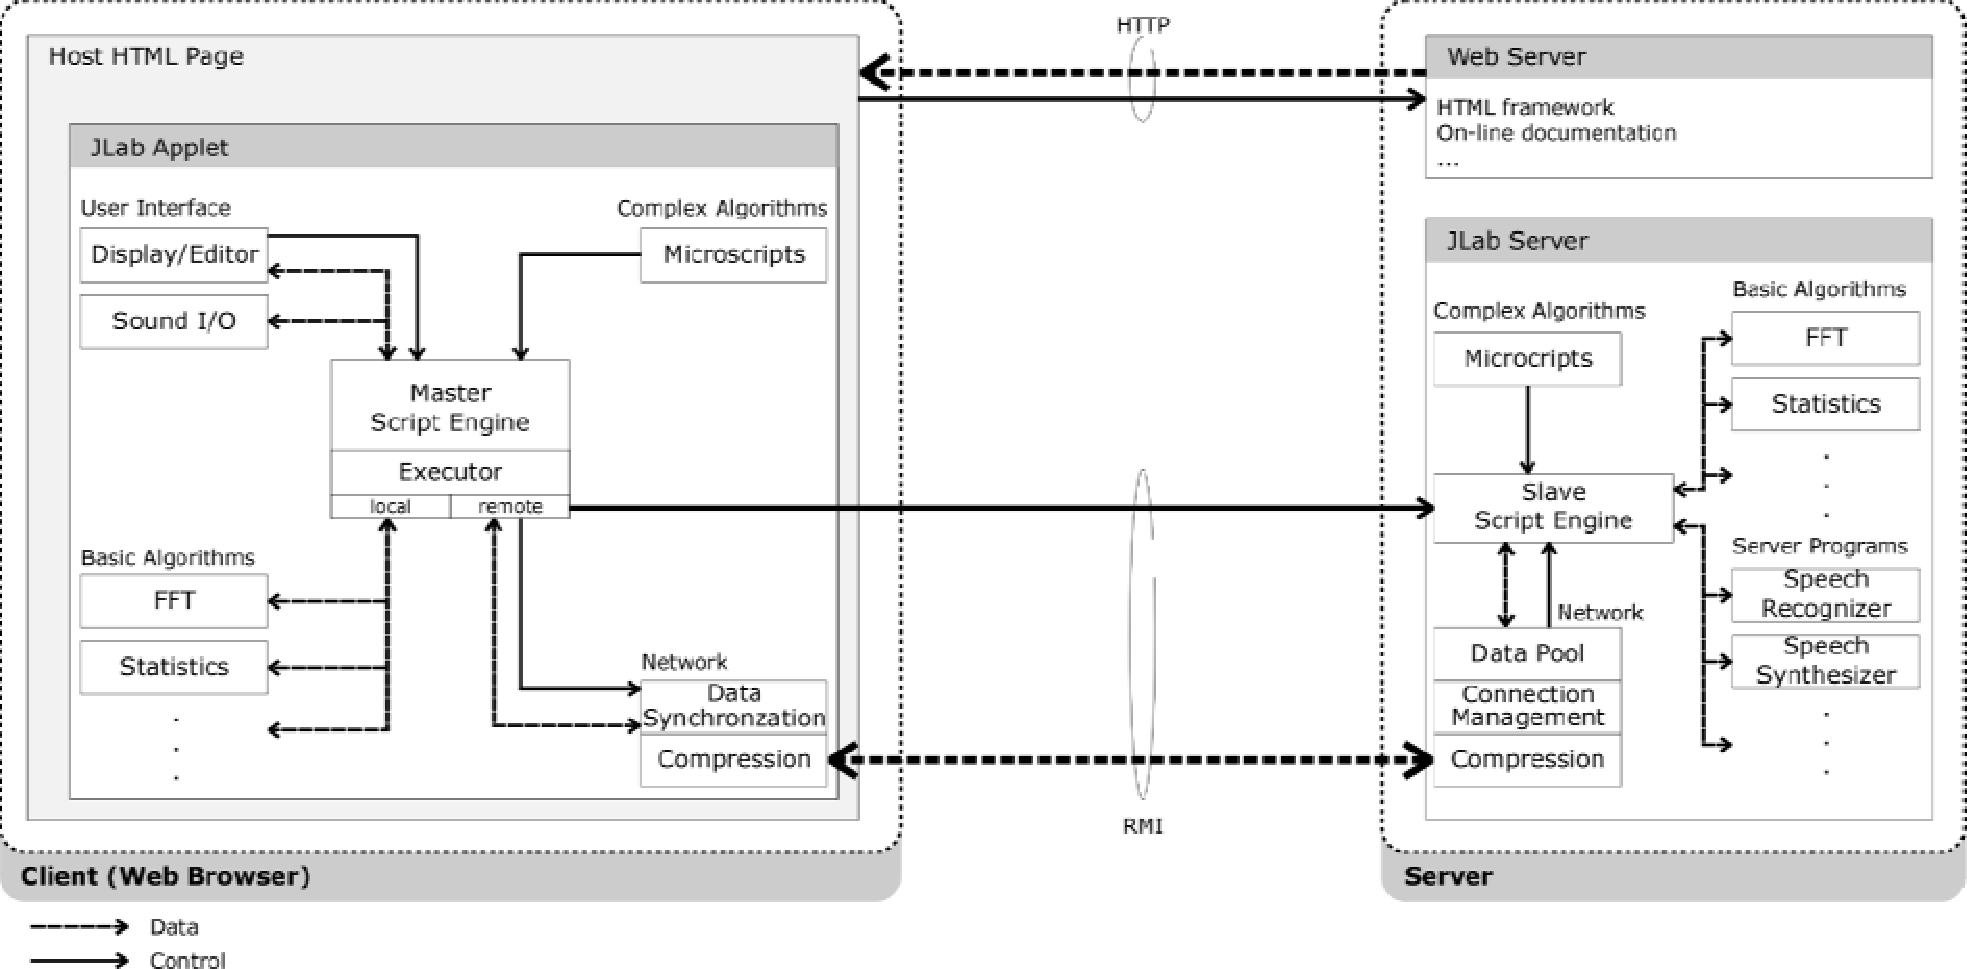
\includegraphics[scale=.45]{abbildung_1}
  \caption{Systemarchitektur der Entwicklungsumgebung}
  \label{fig:abbildung_1}
\end{figure}

\section{Überschrift 1. Ordnung: Times New Roman, 14pt, fett}

\subsection{Überschrift 2. Ordnung: Times New Roman, 12pt, fett}

\subsubsection{Überschrift 3. Ordnung: Times New Roman, 12pt, normal}

Textkörper: Times New Roman, 12pt, normal, Blocksatz

\nocite{2003_ESSV_MM}
\nocite{Fellbaum1999}

\bibliographystyle{essv}
\bibliography{essv}

\end{document}
